%% 
%% Copyright 2019-2021 Elsevier Ltd
%% 
%% This file is part of the 'CAS Bundle'.
%% --------------------------------------
%% 
%% It may be distributed under the conditions of the LaTeX Project Public
%% License, either version 1.2 of this license or (at your option) any
%% later version.  The latest version of this license is in
%%    http://www.latex-project.org/lppl.txt
%% and version 1.2 or later is part of all distributions of LaTeX
%% version 1999/12/01 or later.
%% 
%% The list of all files belonging to the 'CAS Bundle' is
%% given in the file `manifest.txt'.
%% 
%% Template article for cas-sc documentclass for 
%% single column output.

\documentclass[a4paper,fleqn]{cas-sc}
% Use to make nonmenclature
\usepackage{framed} % Framing content

\usepackage{multicol} % Multiple columns environment
\usepackage{amsmath}
\usepackage{nomencl} % Nomenclature package
\usepackage{subcaption}
\makenomenclature

\setlength{\nomitemsep}{-\parskip} % Baseline skip between items

\renewcommand*\nompreamble{\begin{multicols}{2}}

\renewcommand*\nompostamble{\end{multicols}}
% If the frontmatter runs over more than one page
% use the longmktitle option.

%\documentclass[a4paper,fleqn,longmktitle]{cas-sc}
\addtolength{\jot}{3mm}
\usepackage[numbers]{natbib}
%\usepackage[authoryear]{natbib}
%\usepackage[authoryear,longnamesfirst]{natbib}

%%%Author macros
\def\tsc#1{\csdef{#1}{\textsc{\lowercase{#1}}\xspace}}
\tsc{WGM}
\tsc{QE}
%%%

% Uncomment and use as if needed
\newtheorem{theorem}{Algorithm}
\newtheorem{lemma}[theorem]{Lemma}
%\newdefinition{rmk}{Remark}
%\newproof{pf}{Proof}
%\newproof{pot}{Proof of Theorem \ref{thm}}

\begin{document}
\let\WriteBookmarks\relax
\def\floatpagepagefraction{1}
\def\textpagefraction{.001}

% Short title
\shorttitle{}    

\shortauthors{B.T. Rawlins et el.}  
%
%
%\begin{table*}[!t]   
%
%\begin{framed}
%
%\nomenclature{$abbreviation$}{explanation for the abbreviation}
%\nomenclature{$CFD$}{Computational Fluid Dynamics}
%\nomenclature{$u,\,\,\,[m/s]$}{Directional velocity}
%\nomenclature{$p,\,\,\,[Pa]$}{Pressure}
%\nomenclature{$E,\,\,\,[J/kg]$}{Total energy}
%\nomenclature{$Y_k,\,\,\,[kg/kg]$}{Mass fraction of species $k$}
%\nomenclature{$T_g,\,\,\,[K]$}{Gas temperature}
%\nomenclature{$\lambda,\,\,\,[W/mK]$}{Thermal conductivity}
%\nomenclature{$\mu,\,\,\,[Pa.s]$}{Viscosity}
%\nomenclature{$S,\,\,\,[kg/m^3]$}{Mass source term}
%\nomenclature{$S_m,\,\,\,[N/m^3]$}{Momentum source term}
%\nomenclature{$S_h,\,\,\,[W/m^3]$}{Energy source term}
%\nomenclature{$S_k,\,\,\,[kg/m^3]$}{Species source term}
%\nomenclature{$J_k,\,\,\,[kg/m^3]$}{Diffusion flux of species $k$}
%\nomenclature{$\rho,\,\,\,[kg/m^3]$}{Gas density}
%\nomenclature{$\rho_{eff},\,\,\,[kg/m^3]$}{Effective density}
%\printnomenclature
%
%\end{framed}
%
%\end{table*}

% Main title of the paper
\title [mode = title]{Validation of an integrated data-driven surrogate model and a thermo-hydraulic network based model to determine thermal response of a 620 $MW_e$ utility scale boiler using a fully connected mixture density network}  

% Title footnote mark
% eg: \tnotemark[1]
%\tnotemark[<tnote number>] 

% Title footnote 1.
% eg: \tnotetext[1]{Title footnote text}
%\tnotetext[<tnote number>]{<tnote text>} 

% First author
%
% Options: Use if required
%\author[1,3]{Author Name}[type=editor,
%       style=chinese,
%       auid=000,
%       bioid=1,
%       prefix=Sir,
%       orcid=0000-0000-0000-0000,
%       facebook=<facebook id>,
%       twitter=<twitter id>,
%       linkedin=<linkedin id>,
%       gplus=<gplus id>]

\author[1]{B.T. Rawlins}

% Corresponding author indication
\cormark[1]
\cortext[1]{Corresponding author}
% Footnote of the first author
%\fnmark[<footnote mark no>]

% Email id of the first author
\ead{rwlbra001@myuct.ac.za}

% URL of the first author
%\ead[url]{<URL>}

% Credit authorship
% eg: \credit{Conceptualization of this study, Methodology, Software}
\credit{Methodology, Software, Validation, Formal analysis, Investigation,Writing original draft, Visualization.}

% Address/affiliation
\affiliation[1]{organization={Department of Mechanical Engineering, Applied Thermal-Fluid Process Modelling Research Unit, University of Cape Town},
            addressline={Library Road, Rondebosch}, 
            city={Cape Town},
%          citysep={}, % Uncomment if no comma needed between city and postcode
            postcode={7701}, 
            %state={},
            country={South Africa}}

\author[2]{Ryno Laubscher}[]

% Footnote of the second author
%\fnmark[2]

% Email id of the second author
%\ead{rlaubscher@sun.ac.za}
% URL of the second author
%\ead[url]{}
% Credit authorship
\credit{Writing review \& editing, Methodology, Resources, Conceptualization.}
% Address/affiliation
\affiliation[2]{organization={Department of Mechanical Engineering, Stellenbosch University},
            addressline={Banghoek Road, Stellenbosch}, 
            %city={Stellenbosch},
%          citysep={}, % Uncomment if no comma needed between city and postcode
            postcode={7600}, 
            %state={},
            country={South Africa}}
% Footnote text
%\fntext[1]{}
% For a title note without a number/mark
%\nonumnote{}
\author[1]{Pieter Rousseau}
% Email id of the second author
%\ead{pieter.rousseau@uct.ac.za}
% Credit authorship
\credit{Writing review \& editing, Resources, Conceptualization}

% Corresponding author text

% Here goes the abstract
\begin{abstract}
An integrated data-driven surrogate model and 1-dimensional (1D) process model of a 620 $MW_e$ utility scale boiler was developed. A robust and computationally inexpensive computational fluid dynamic (CFD) model of the utility boiler was utilized to generate the solution dataset for surrogate model training and testing. In the present work, a standard multi-layer perception (MLP) and MLP connected mixture density network (MLP-MDN) machine learning architectures are compared for use as a surrogate model to predict the boilers' heat exchanger heat loads and the flue-gas inlet conditions to the convective pass. A hyperparameter search was performed to find the best MLP and MLP-MDN architecture, with the MLP-MDN model being capable of predicting the uncertainty. The MLP-MDN showed approximately a 20\% decrease in the mean absolute error (MAE) and was selected for surrogate model integration. Validation of the integrated model against plant data was performed for a wide range of loads. Sufficient resolution of the thermal-hydraulic response was observed for all load ranges with a 5-8\% error discrepancy. The validated model was subsequently used to investigate the effects of using a poor quality fuel for the 100\% maximum continuous rating (MCR) load case. The results show that poor quality fuel leads to a lower operational efficiency for the same operational inputs.
\end{abstract}

% Use if graphical abstract is present
%\begin{graphicalabstract}
%\includegraphics{}
%\end{graphicalabstract}

% Research highlights
\begin{highlights}
\item Data-driven surrogate model development using CFD solution data.
\item 1-D process and surrogate model integration.
\item Development of mixture density network using simulation data.
\end{highlights}

% Keywords
% Each keyword is seperated by \sep
\begin{keywords}
Mixture density network \sep data-driven surrogate modelling \sep Computational fluid dynamics \sep
\end{keywords}

\maketitle

% Main text
\section{Introduction}\label{intro}
A significant portion of the developing world, including South Africa, rely on the use of conventional coal fired power plants to meet the local energy demand \cite{Rousseau2020}. However, international relief and pressure have lead to many renewable energy sources being implemented worldwide. The increasing penetration of renewable energy sources onto the current electrical grids is predicted to push conventional base-load thermal power plants to operate on a mid-merit basis. The mid-merit operation requires these power plants to operate flexibly, with faster ramping and start-up rates \cite{Safdarnejad2019}. This can result in an increase in the thermal stresses on key operational components due to the changes in heat loads \cite{Modlinski2019}. Therefore it is important to be able to predict the thermal-hydraulic response of these components at off design conditions.\\

Computational fluid dynamics (CFD) aligns itself well for the analysis of solid fuel combustion systems, providing sufficient resolution of the fluid flow, particle concentration and heat transfer characteristics. Simulations using CFD predominately explore the effects that the flue-gas has on the overall system, investigating pollutant limits \cite{Liu2021}, design optimization \cite{dugum2019, Gu2020} and particle effects \cite{Laubscher2020}. The associated computational burden limits the use of CFD for steady-state analysis for industrial sized systems. However, the use of a multiphase modelling approach has been shown by researchers Rawlins et al \cite{Rawlins2022} to reduce the computational effort by approximately 25\%.\\

Investigating the thermal-hydraulic response requires the use of 1-D process modelling to capture the steam/water cycle, since the 3-D simulation of the working fluid network would amount to a drastic increase in the computational demand. Co-simulation techniques involve the use of both 3-D CFD models and 1-D process models to investigate operational limits. Rousseau and Laubscher \cite{Rousseau2020} used the methodology to investigate the effects high ash quality fuel has on the heat absorption of the radiant superheaters (SHs). The feasibility of co-simulation models rely on the integration of the two models and are limited to steady state applications.\\

Negating the high computational burden, data-driven surrogate models are typically utilized. Data driven surrogate models form part of statistical regression models, where the true objective function is namely fitted using true evaluations of the objective function \cite{Wheeler2019}. Artificial neural networks (ANNs) are one of the main machine learning algorithms/techniques to facilitate the learning process, other procedures include Kriging models \cite{Fei2015} and support vector machines \cite{Lv2017}.\\

The works of Singh and Abbassi \cite{Singh2018} incorporated the use of an ANN and CFD model to investigate the transient thermal modelling of an off-highway machinery cabin. The ANN training data was obtained from a 1-D process model for the refrigeration cycle. The methodology was successfully able to integrate the ANN capabilities with a 3-D CFD simulation model negating the need for a coupled simulation procedure. Similary, Fei et al \cite{Fei2015} made use of a fast set of reduced order models (ROMs), using the Kriging method, based off of CFD data to investigate the retrofitting of coal fired power plant under oxy-fuel conditions. Using an integrated ROM to process model, a range of air-coal conditions where investigated, with the model illustrating sufficiently accurate results. However no operational uncertainty was not incorporated into the input parameters to account for real world operational effects (disturbances, local atmospheric conditions etc.).\\

The importance for predicting and acknowledging system/load uncertainties in conventional coal fired power plants are paramount for the safe operation and maintenance of these plants \cite{Madejski_18}. The uncertainty associated with a thermal power plants operational parameters such as fuel quality, combustion processes, and  burner biasing can lead to significant changes in the thermal-hydraulic response \cite{Sarkar2015}. The design space load uncertainty of a combined cooling, heating and power system was investigated by Lu et al \cite{Lu2021}. Using a multi-objective optimization model, factors such as pollutant emission, economy and the system reliability were incorporated to improve the operational performance. The model illustrated its future use for designers in providing the best configuration scheme under system load uncertainties.\\ 

It is noted that CFD cannot meet the real time requirement for on line performance monitoring, due to the complex solving mechanisms and time-consuming calculations. However, it is a feasible alternative to generate training and testing datasets for ANN implementation, since using CFD does not interfere with normal operation of the plant. In addition to this a wider range of appropriate operating conditions can be simulated.\\
 
In the present work, an integrated data-driven surrogate model and 1-D process model was proposed to investigate the thermal response of a 620 $MW_e$ utility scale boiler. A steady-state multiphase CFD model was developed for the 620 $MW_e$ utility scale boiler under investigation and was used to generate a simulation dataset for a 180 different input conditions. To establish the data-driven surrogate model complexity, various ANN frameworks were considered, namely a standard MLP and a MLP-MDN, where the latter allows the introduction of uncertainty into the model predictions. A hyper-parameter search was conducted to establish the best performing model, with the lowest MAE being an essential criterion. Validation of the integrated surrogate and process model was performed for maximum continuous ratings (MCR) for the 100\%, 80\% and 60\% load ranges where measured data was made available. Subsequently the use of the validated model to investigate poor fuel quality at 100\% MCR was conducted, where the ash and moisture contents where varied for two separate cases.

\section{Applicable machine learning theory}
The present work makes use of various machine learning architectures to develop a surrogate model that can predict the thermal and combustion characteristics of a utility scale boiler using high level inputs. The current section discusses the details of the respective architectures, namely linear regression, ANN and MLP-MDN models.  
\subsection{Linear regression}
The present work makes use of a multiple linear regression model as a base model for comparative purposes in the validation case study of Section \ref{sec_result_1}. The main assumption of a multiple linear regression model is that the output/s can be calculated from a linear combination of the variable inputs. In other words a linear regression models aims to determine the quantitative relationship between the dependent and independent variables \cite{Wen2022}. The representation of the $i$-th dependent variable ($y_i$) can be written as follows for $m$-number of independent variables ($x_{mi}$):
\begin{equation}
\begin{split}
&y_i = \beta_0+\beta_1x_{1i}+...+\beta_mx_{mi}\\
&i = 1,2,3...n
\end{split}
\end{equation}
where $\beta_0$ is a constant term, $\beta_{m}$ is the $m$-th coefficient, and $n$ is the total number of observations.\\
 
The optimal solution can be estimated by minimizing the cost function ($J$). A cost function usually calculates the difference between the estimated and the desired values and is reported as a single number. Multiple linear regression problems namely utilize the mean square error (MSE) between the desired and estimated ($\hat{y_i}$)  values \cite{Wheeler2019}, which is given in Equation \ref{eqn_lin_cost}.
 \begin{equation}\label{eqn_lin_cost}
J_{MSE}=\frac{1}{n}\sum^n_{i=1}(y_i-\hat{y_i})^2
\end{equation} 

To minimize the cost function, the gradient descent algorithm is the preferred method \cite{Wen2022}, which is an iterative procedure used to find the local minimum/maximum. Considering the cost function as a function of the weight the algorithm can be written as shown in Equation \ref{eqn_grad_descent}.  
\begin{equation}\label{eqn_grad_descent}
\beta_{m} = \beta_m-\eta\frac{\partial}{\partial\beta_m}J(\beta_m)
\end{equation}
where $\eta$ is known as the learning rate.\\

In most cases the relationship between the dependent and independent variables are not always linear. Special linear basis models, such as polynomial, sinusoidal and radial can be used to optimize the training results \cite{Rasmussen2006}. For the current work a multiple linear progression model is utilized as a base model for comparison in Section \ref{sec_result_1}. 
\subsection{Multilayer perception networks}
Artificial neural networks (ANN) are machine learning systems inspired by biological animal brains \cite{Rasmussen2006}. There are many classifications of ANNs, with multilayer perception networks (MLP) being the standard representation \citep{goodfellow}. Typically MLPs are adapted for supervised learning problems where the input variables are mapped to labelled output variables. The relationship between the input and output variables are learned by optimizing the weights ($\overline{w}$) and biases ($\overline{b}$) to minimize a selected cost function, which for most cases is the MSE given in equation \ref{eqn_lin_cost}. A standard MLP schematic is given in figure \ref{fig_mlp_schematic}, illustrating the common features of a MLP, that being the input, hidden and output layers.\\
\begin{figure}[h!]
	\centering
		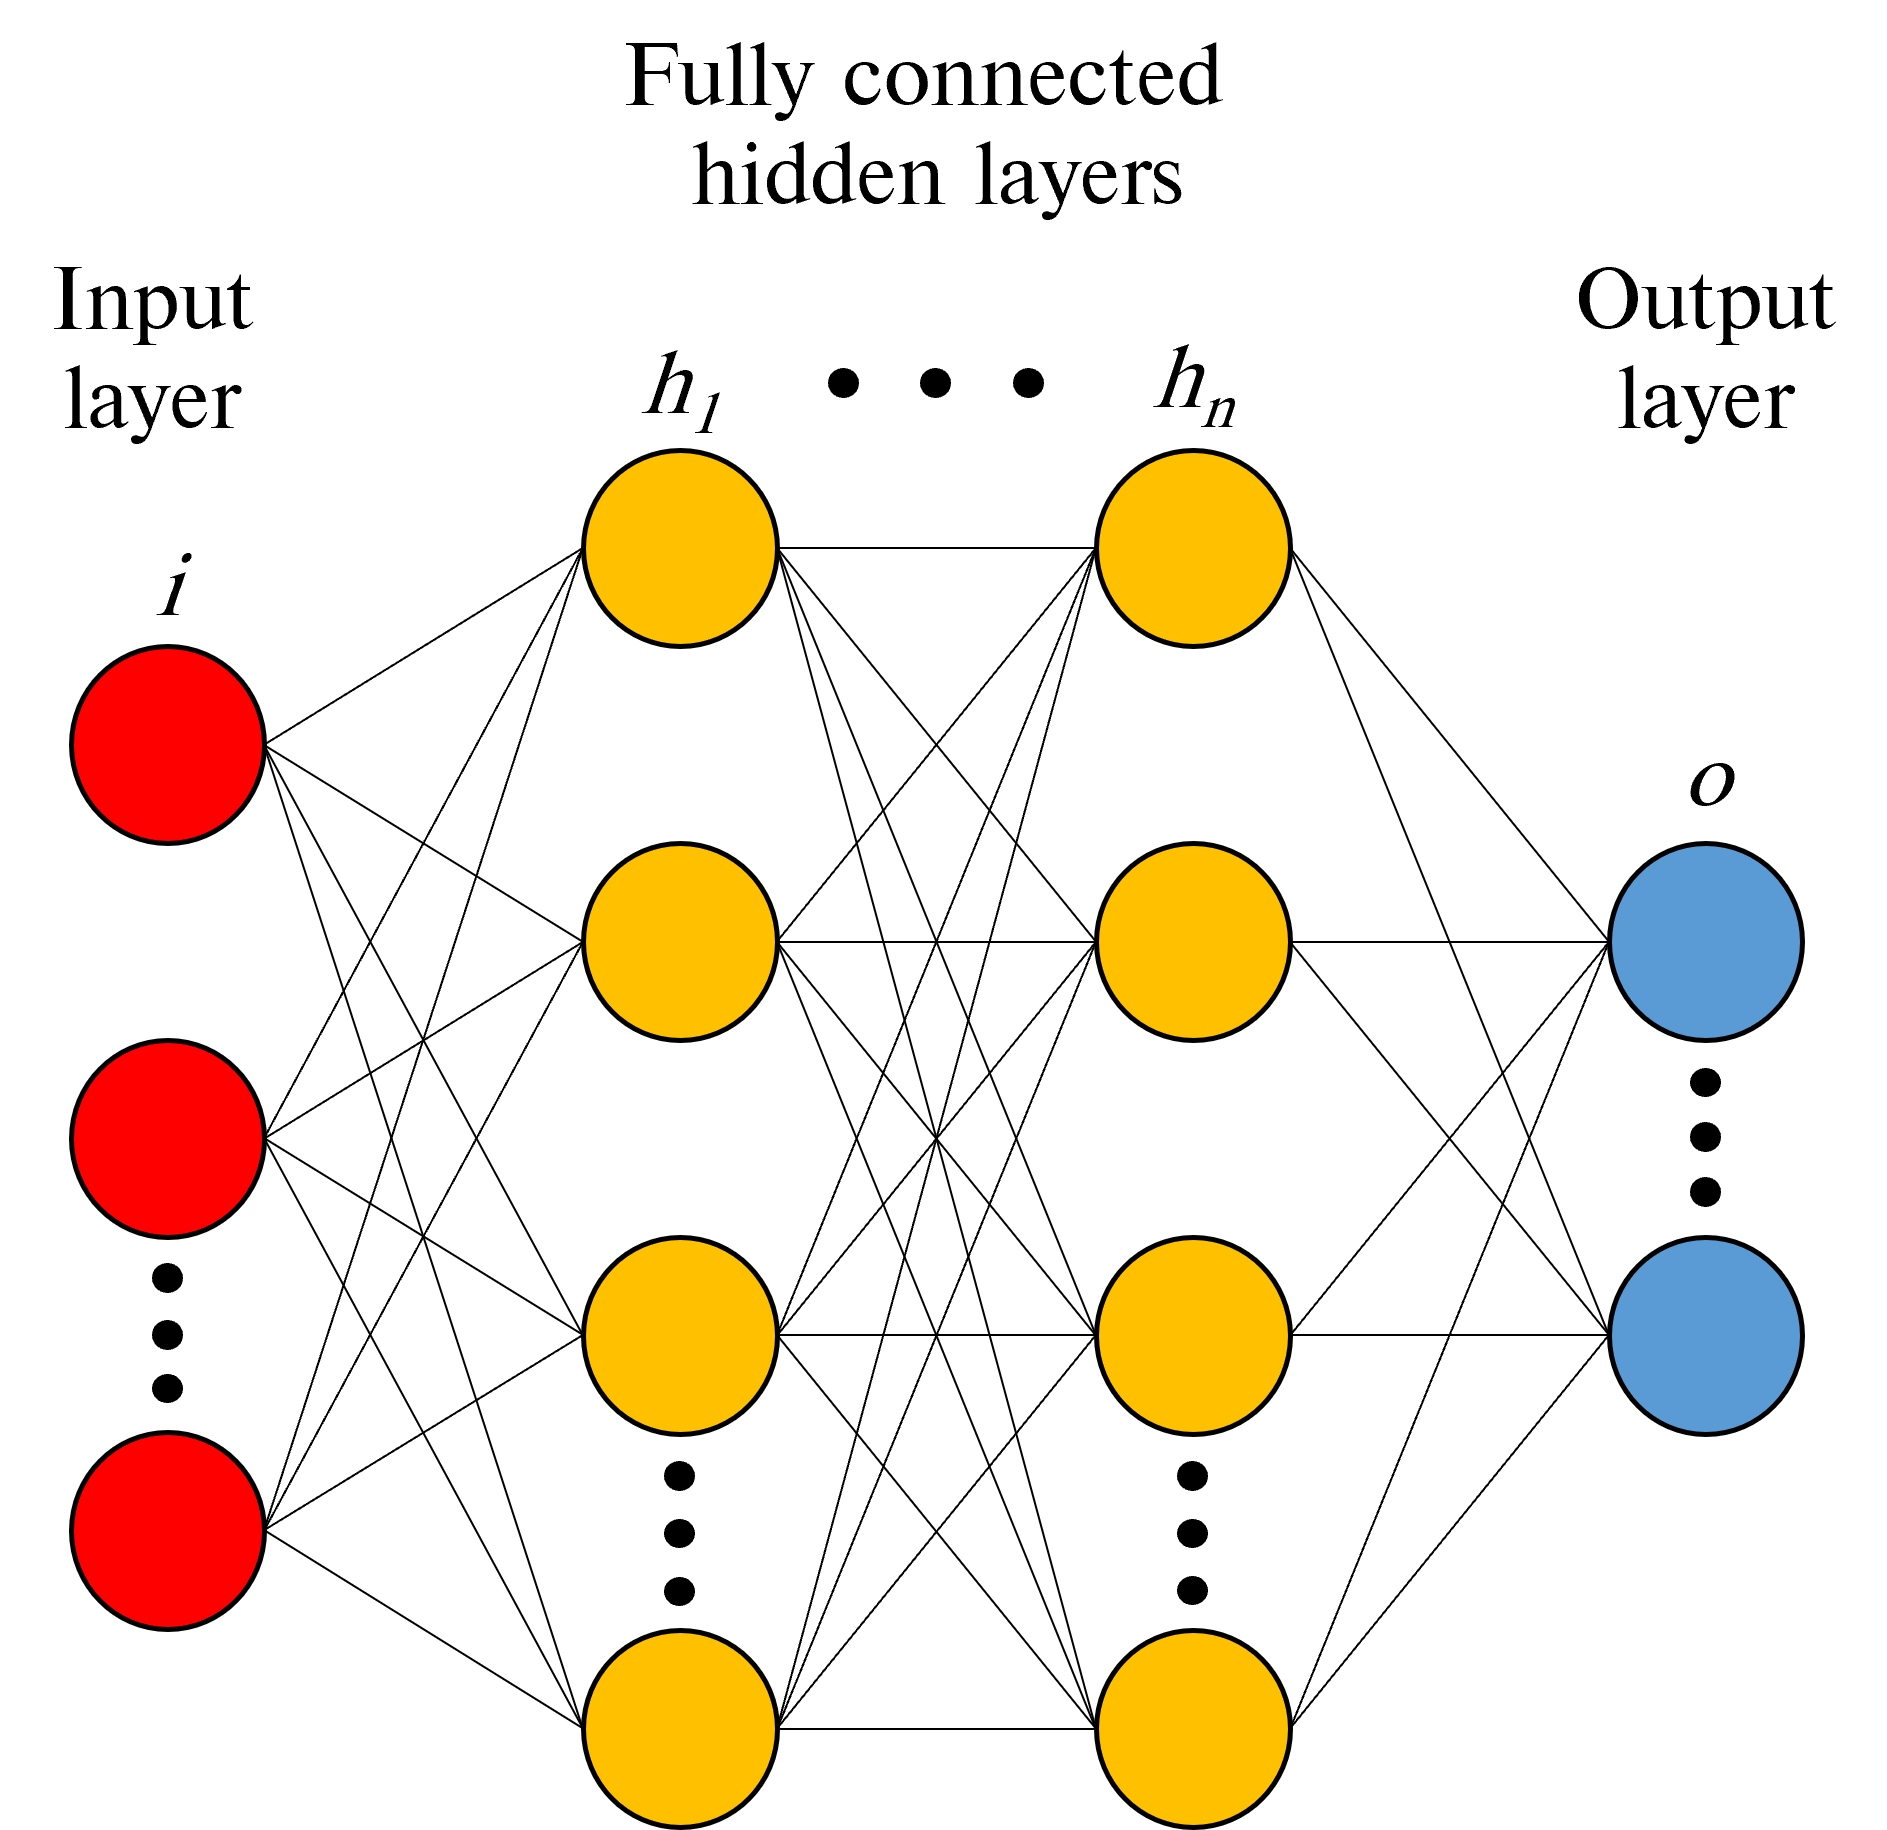
\includegraphics[scale=0.5]{ML_SCHEMATIC}
	  \caption{Traditional MLP schematic}\label{fig_mlp_schematic}
\end{figure}

To calculate the output values ($\hat{y_i}$) the forward propagation algorithm is utilized, which calculates the output for each layer and moves sequentially through the network till an output is determined. Each network layer output is calculated using two steps, the first being the calculation of the summed signal $\overline{z}_l$ and secondly the use of an activation function to generate the output signal $\overline{h}_l$. Equation \ref{eqn_summed_sig} highlights the first step, where $\overline{h}_{l-1}$ is the output signal from the previous layer.
\begin{equation}\label{eqn_summed_sig}
\overline{z}_l = \overline{h}_{l-1}\cdot\overline{w}_l+\overline{b}_l
\end{equation}

The result of the equation \ref{eqn_summed_sig} is subsequently passed to an activation function ($\overline{h}_l = \sigma_l(\overline{z}_l)$). There are various activation functions that can be utilized, such as linear, ReLu, Elu, and the hyperbolic-tangent \citep{goodfellow}, with the final layer activation function usually being linear for regression models. The current work makes use of ReLu and linear activation functions for the hidden layers. The ReLu and linear activation functions are shown in Equation \ref{eqn_act_func}.
\begin{equation}\label{eqn_act_func}
\begin{split}
&\overline{h}_l=\sigma_{ReLu}(\overline{z}_l) = \overline{z}_l =  
	\begin{cases}
	 \overline{h}_{l-1}\cdot\overline{w}_l+\overline{b}_l\,\, &if\,\,\,\, \overline{z}_l>0\\
	 0\,\, &if\,\,\,\, \overline{z}_l<0
	\end{cases}\\
&\overline{h}_l=\sigma_{linear}(\overline{z}_l) = \overline{z}_l = \overline{h}_{l-1}\cdot\overline{w}_l+\overline{b}_l
\end{split}
\end{equation}

When the forward propagation step is complete, the network weights and biases can be updated to minimize the cost function (refer to Equation \ref{eqn_lin_cost}) using the backward propagation method \cite{Rumelhart1986}. The methodology calculates the gradient of the cost function with respect to the weights and biases for each layer. Once the gradients have been calculated the weights and biases are updated using the gradient descent algorithm. The current work makes use of the Adam \cite{goodfellow} alternative to the gradient descent algorithm and is illustrated in Equation \ref{eqn_adam_algor}. Forward- and backward-propagation algorithms would be iteratively conducted until the cost function is reduced to below a desired threshold.

\begin{theorem} 
\begin{equation}\label{eqn_adam_algor} 
\begin{split}
&\overline{m}\leftarrow \beta_1\overline{m}+(1-\beta_1)\nabla_{\theta}J_{MSE}(\overline{\theta})\\
&\overline{s}\leftarrow \beta_1\overline{s}+(1-\beta_2)\nabla_{\theta}J_{MSE}(\overline{\theta})\otimes&\nabla_{\theta}J_{MSE}(\overline{\theta})\\
&\overline{m}\leftarrow\frac{\overline{m}}{1-\beta_1^t} \\
&\overline{s}\leftarrow\frac{\overline{s}}{1-\beta_2^t}\\
&\overline{\theta}\leftarrow\overline{\theta}-\eta\overline{m}\otimes(\sqrt{\overline{s}+\epsilon})^{-1}\\
\end{split}
\end{equation}
\end{theorem}

The variable $\bar{\theta}$, of Equation \ref{eqn_adam_algor}, represents the model parameters weights ($\bar{w}$) and biases ($\bar{b}$) for each layer. Scaling ($\bar{s}$) and momentum ($\bar{m}$) matrices are initialized to zero when beginning the training phase, $t$ is the iterative counter, $\beta_1$ and $\beta_2$ are the momentum and scaling decay hyper-parameters set to values of 0.9 and 0.999 respectively. Lastly $\epsilon$ is a smoothing term set to a value of $10^{-8}$.

\subsection{Mixture density networks (MDNs)}
Mixture density networks are fundamentally built from two components, that being an ANN and a mixture model, this allows for multi-modal predictions. The ANN can be a standard feed-forward MLP or a recurrent neural network (RNN), with RNNs traditionally being used in dynamic applications with at least one feedback loop \citep{Oko2015}. For this study the traditionally MLP is used.\\

MDNs are used to predict the parameters of a probability distribution ($P(\overline{X}\mid\overline{Y})$) allowing for non-Gaussian distributions to be modelled, thus making MDNs a probabilistic machine learning framework. MDNs estimate the conditional probability distribution as a mixture of Gaussian distributions where the mixing coefficients ($\overline{\pi}_k$) and component densities are flexible functions of the input data ($\overline{X}$). Equation \ref{eqn_cond_prob_func} illustrates the conditional probability function.
\begin{equation}\label{eqn_cond_prob_func}
P(\overline{X}\mid\overline{Y}) = \sum_{k=1}^K\pi_k(\overline{X})\cdot \mathbb{N}(\overline{Y}\mid \overline{\mu}_k(\overline{X}),\overline{\sigma}^2_k(\overline{X}))
\end{equation}
where $K$ represents the number of selected normal distributions, while $\overline{\mu}_k$ and $\overline{\sigma}^2_k$ are the predicted means and variances for each distribution $k$ given the input data $\overline{X}$ respectively.\\

A schematic of a simple MLP-MDN network is given in Figure \ref{fig_mdn_schematic}, highlighting the mixing coefficients, predicted means and deviations. It can is shown that modifications are made to the output layer by splitting the network output into three parts in order to calculate the $\overline{\pi}_k$, $\overline{\mu}_k$ and $\overline{\sigma}^2_k$ for each $k$ distribution. This enables the MDN network to learn the $P(\overline{X}\mid\overline{Y})$.\\

\begin{figure*}[h!]
	\centering
		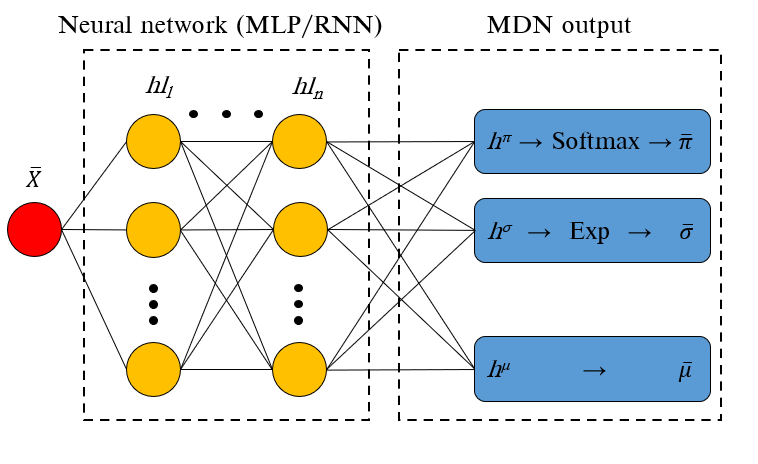
\includegraphics[scale=0.5]{MDN_SCHEMATIC}
	  \caption{Simple MLP-MDN network}\label{fig_mdn_schematic}
\end{figure*}

Bishop \cite{bishop1994} proposed the following restrictions for the mixing coefficients and variance components of the MDN output layer. Since the mixing coefficients contain the discrete probabilities of an output belonging to each $K$ normal distribution for all observations, the mixing coefficients must satisfy the constraints listed in Equation \ref{eqn_mix_coef_constraint}.
\begin{equation}\label{eqn_mix_coef_constraint}
\begin{split}
&\sum_{k=1}^K\overline{\pi}_k^n=1\\
&0\leq\overline{\pi}_k^n\leq1
\end{split}
\end{equation}
These constraints are met by using a Softmax function on the output of the hidden layer $h^{\pi}$. The mixing coefficient is calculated using Equation \ref{eqn_mix_coeff}.
\begin{equation}\label{eqn_mix_coeff}
\overline{\pi}_k^n(\overline{x}^n)=\frac{exp(h_k^{\pi,n})}{\sum_{k=1}^Kexp(h_k^{\pi,n})}
\end{equation}

Similarly a constraint is applied to the standard deviation values ensuring a positive value, this is achieved through the use of an exponential function being applied to the standard deviation leg of the MDN output layer, namely $h^{\sigma}$. Equations \ref{eqn_stddev} shows the imposed constraint for the standard deviation leg.\\
\begin{equation}\label{eqn_stddev}
\begin{split}
&(\overline{\sigma}^n_k(\overline{x}^n))^2\geq 0\\
&\sigma_k^n(\overline{x}^n)=exp(h_k^{\sigma,n})
\end{split}
\end{equation}

The MDN weights and biases are optimized by minimizing the negative log-likelihood for all observations in a batch, this is shown in Equation \ref{eqn_nll}.

\begin{equation}\label{eqn_nll}
J_{NLL}(\overline{Y},\overline{\pi},\overline{\sigma},\overline{\mu})=-\sum^N_{n=1}ln\left\{\sum^K_{k=1}\overline{\pi}_k(\overline{X}^n,\overline{\theta})\cdot \mathbb{N}(\overline{Y}^n\mid\overline{\mu}_k(\bar{X}^n,\bar{\theta}),\overline{\sigma}^2_k(\overline{X}^n,\overline{\theta})) \right\}
\end{equation}


\section{Data generation}
A steady-state multiphase non-thermal equilibrium CFD model was used to generate the target data, which was subsequently used for training/testing of an appropriate surrogate model.

\subsection{CFD model setup}
The current study makes use of the commercial CFD software package ANSYS\textsuperscript{\textregistered} Fluent 2019 R3 to resolve the fluid flow, heat transfer and combustion processes for a 620$MW_e$ utility scale coal fired boiler. The computational domain is modelled on a symmetry plane half way through the depth of the boiler. Figure \ref{fig_cfd_geom_bc} highlights the computational domain and defines the important boundary conditions.\\ 

\begin{figure*}[h!]
	\centering
		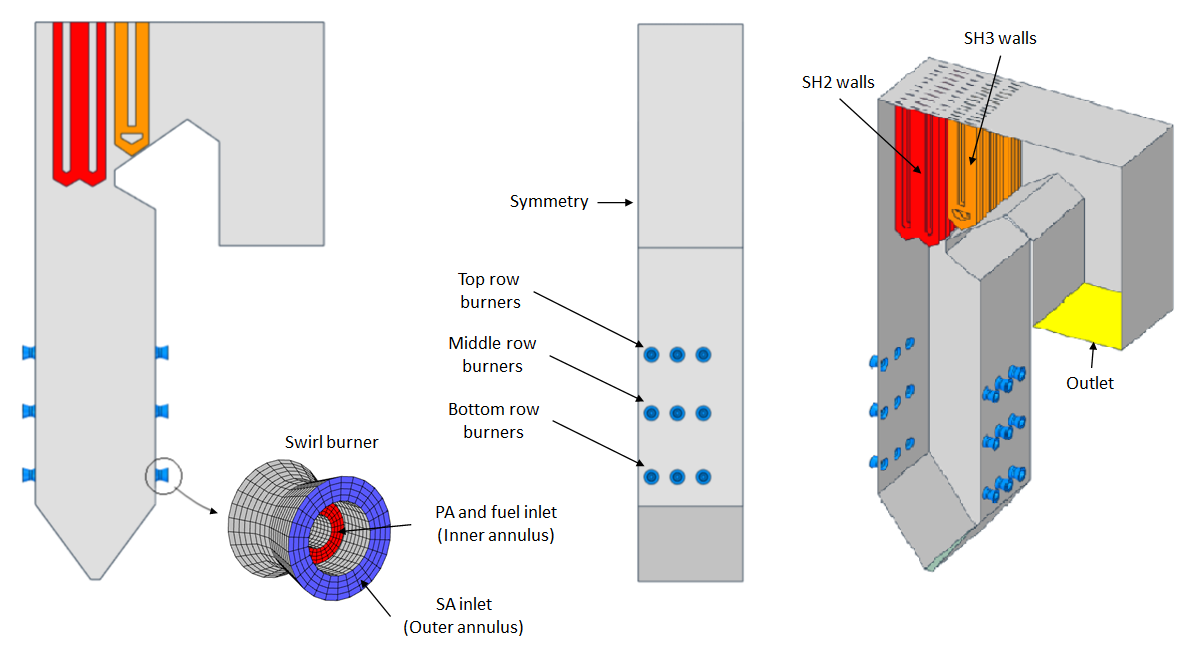
\includegraphics[scale=0.4]{CFD_GEOMETRY}
	  \caption{CFD model geometry and boundary condition descriptions.}\label{fig_cfd_geom_bc}
\end{figure*}

The general conservation equations, which include, continuity, momentum, energy and species, were solved using a Eulerian approach. The subsequent equations are stated in Equation (\ref{eqn_cfd}).

\begin{flalign} \label{eqn_cfd}
&\frac{\partial}{\partial x_{i}}(\rho \bar{u}_{i})=S \nonumber &&\\
&\frac{\partial}{\partial x_{i}}(\rho_{eff} u_{i}u_{j})+\frac{\partial \overline{p}}{\partial x_{j}}= \nonumber&&\\
&\frac{\partial}{\partial x_{i}}\left[\mu\left\{\frac{\partial u_{j}}{\partial x_{i}}+\frac{\partial u_{i}}{\partial x_{j}}-\frac{2}{3}\delta_{ij}\frac{\partial u_{i}}{\partial x_{i}}\right\}\right]+\frac{\partial}{\partial x_{i}}(-\rho\overline{u_{i}^{'}u_{j}^{'}})+S_m \nonumber \nonumber &&\\
&\frac{\partial }{\partial x_{i}} (u_{i}[\rho E+p])=\frac{\partial }{\partial x_{j}}\left[\lambda\frac{\partial T_{g}}{\partial x_{j}}\right] +S_{h} &&\\
&\frac{\partial}{\partial x_{i}}(\rho u_{j}Y_{k})=-\frac{\partial}{\partial x_{j}}(\vec{J_{k}})+ \sum_r R_{j,r} + S_{k} \nonumber && 
\end{flalign}

The resolution of the Reynolds stress term found in the momentum equation, $-\rho\overline{u_{i}^{'}u_{j}^{'}}$, was approximated using the Boussineq equation \citep{Versteeg2007}. In the present study the realizable k-$\varepsilon$ turbulence model was utilized to address the turbulence closure problem, this model was selected for its applicability in modelling the effects of coal-fired swirl burners \citep{Modlinski2010}.\\

The P1 radiation model was used to resolve the radiative field in the domain. Particle transport was modelled using a multiphase approach, further details on the approach are provided in the validation study of Rawlins et al \citep{Rawlins2021}. The combustion follows a four step sequential process, beginning with the heating and evaporation of the moisture present in the fuel, followed by the devolatilization process where the volatiles are liberated from the solid particle, succeeded by the phenomena of char burnout, and finally the gas phase reactions would commence. The char oxidation reaction product species was set to that of carbon monoxide ($CO$). For the gas-phase reactions the turbulence-chemistry interaction was approximated using the eddy dissipation model (EDM). A summary of the combustion equations and constants are provided in Table \ref{tbl_combust}.\\

\begin{table*}[h!]
\caption{Summary of combustion models and constants used in the CFD model}\label{tbl_combust}
\begin{tabular*}{\tblwidth}{p{0.325\textwidth}p{0.35\textwidth}p{0.25\textwidth}}
\toprule
Model & Equation/s & Constant/s\\
\midrule
\multicolumn{3}{l}{\textit{Devolatilization}} \\ % Table header row
Single rate kinetic model &$\frac{dm_{vol}}{dt} = R_{vol}(m_{0,vol}-m_{vol})$,  & $A_{vol} = 2\times10^5 [s^{-1}]$, \\
& $R_{vol} = A_{vol}exp\left(\frac{E_{a,vol}}{RT_p}\right)$ & $ E_{a,vol} = 6.7\times10^7 [J/kmol]$ - \cite{Sheng2004} \\
\multicolumn{3}{l}{\textit{Char oxidation}} \\
Diffusion/kinetic - \citep{Baum1971} & $\frac{dm_{char}}{dt} = -A_p p_{O_{2}} \frac{R_{diff}R_c}{R_{diff} + R_c}$,  & $A_{c} = 0.0053 [kg/m^2sPa]$, \\
& $R_{c} = A_{c}exp\left(\frac{E_{a,c}}{RT_p}\right)$,  & $E_{a,c} = 8.37\times10^7 [J/kmol]$ - \cite{Sheng2004} \\
& $R_{diff} = \frac{5\times10^{-12}}{d_p} \left(\frac{T_g+T_p}{2}\right)^{0.75}$&\\
\multicolumn{3}{l}{\textit{Gaseous reactions of volatiles and $CO$}} \\
Eddy dissipation model - \cite{Ansys} & $R_{k,r,P} =\vartheta_{k,r}M_{w,k}AB\rho\frac{\varepsilon}{k}min\left(\frac{\sum_{p} Y_p}{\sum_{j}\vartheta_{j,r}M_{w,j}}\right)$, $R_{k,r,R} =\vartheta_{k,r}M_{w,k}A\rho\frac{\varepsilon}{k}min\left(\frac{Y_R}{\vartheta_{R,r}M_{w,R}}\right)$ & $A=4.0$, $B=0.5$\\
\bottomrule
\end{tabular*}
\end{table*}

The simulations were solved using the SIMPLE pressure–velocity coupling scheme. The pressure term was discretized using the PRESTO! scheme. Momentum, species and energy equations were discretized using the second-order upwind scheme and the turbulent kinetic energy and dissipation rate using the first-order upwind scheme. The numerical mesh was generated using quadrilateral elements consisting of 6 million cells.  The convergence criteria for the simulation model was set to $1\times10^{-3}$ for the continuity equation, $1\times10^{-4}$ for the velocity equations, $1\times10^{-6}$ for the remaining transport equations, and $1\times10^{-4}$ for monitored key parameters.

\subsection{Simulated dataset}
As previously mentioned the aim of this study is to illustrate the use of a data-driven surrogate model, integrated with a 1D process model, to predict the heat loads to the various heat exchanging components, the flue-gas composition and exit gas temperatures for a utility scale boiler using various high-level inputs. The inputs include the the following, the excess air ratio per burner, the total mill flowrate for the six mills in operation, the average steam temperatures for the platen and final superheaters, the fouling resistance for the platen and final superheaters, the composition of ash and moisture of the fuel and the gross calorific value of the fuel. Thus the input field has a dimensionality of $d_{inputs}=14$.\\

A design of experiments (DOE) was conducted to generate a set of 180 simulation cases to obtain a representative set of results. The various model input ranges used in the DOE are given in Table \ref{tbl_doe}. The ranges where selected to cover a wide range of operational loads with maximum continuous ratings (MCR) between 100\% and 30\%. A total of 27 output target values ($d_{targets}$) are realised for each CFD simulation case. Due to the quasi-steady nature of the CFD simulations, output target values for were taken every 50 iterations for the last 2500 iterations for a converged CFD simulation. This results in each CFD simulation case having a data solution matrix size of ($\bar{Y}\in50\times27$).\\

The DOE matrix was populated using the Latin Hypercube Sampling (LHS) method provided in the Python $pyDOE$ library. Once the CFD simulations achieved convergence, the target data, comprising of the discretized heat loads to the furnace, platen and final SHs, the exit flue-gas temperatures and combustion characteristics, was stored for each case. The target dataset was split with 80\% being used for training purposes and the remainder for testing. To reduce the training time of the neural networks a min-max normalization was utilized scaling all the dataset entries to values between $0\rightarrow1$.\\

\begin{table*}[h!]
\caption{Design of experiments input ranges for  simulations}\label{tbl_doe}
\begin{tabular*}{\tblwidth}{p{0.5\textwidth}p{0.15\textwidth}p{0.15\textwidth}p{0.15\textwidth}}
\toprule
 Input variables& Min& Max& Units \\ % Table header row
\midrule
 Total fuel flow rate for mills 1 to 6 & 39.5 & 120.2 & $kg/s$ \\
 Fuel proximate analysis moisture mass fraction, $Y_{H_2O}$ & 0.025 & 0.085 & $kg/kg$ \\
 Fuel proximate analysis ash mass fraction, $Y_{ash}$  & 0.259 & 0.559 & $kg/kg$ \\
 Platen SH fouling thermal resistance, $R_{platen}$  & 0.004 & 0.007 & $m^2K/W$ \\
 Final SH fouling thermal resistance, $R_{final}$  &0.01 & 0.017 & $m^2K/W$ \\
\midrule
Dependent variables& \multicolumn{2}{l}{Function of}& Units\\
\midrule
Higher heating value&\multicolumn{2}{l}{Fuel constituents $Y_{H_2O}$ and $Y_{ash}$}&$J/kg$\\
Excess air & \multicolumn{2}{l}{Total fuel flow rate for mills} & $\%$\\
Platen SH internal steam temperature& \multicolumn{2}{l}{$R_{platen}$} & $K$\\
Final SH internal steam temperature& \multicolumn{2}{l}{$R_{final}$} & $K$\\
\bottomrule
\end{tabular*}
\end{table*}
\section{Model development}
The present work makes use of two types of machine learning models, namely a standard artificial neural network (ANN/MLP) and a mixture density designated model connected to a standard ANN (MLP-MDN). The following section will discuss the hyper parameter tuning and final selected model configuration. The programming language Python 3.7.8 and the Tensorflow machine learning libraries were utilized in the present study. 
\subsection{Model configuration}
The goal of the final machine learning configuration is to be able to predict the heat load distributions to the furnace, platen superheater (SH) and final SH walls, the combustion characteristics and flue-gas temperatures at the exit, using the high level input ranges given in Table \ref{tbl_doe}.\\

The outputs for the MLP will consist of $y=50\times180=9000$ outputs. Thus, for a data batch size, $m_b$, the output tensor for the MLP model will be $\hat{Y}\in \mathbb{R}^{m_b\times y\times 27}$ since $d_{targets}=27$. However, the MDN-ANN models output data will consist of three parts, namely; the mixing coefficients tensor of shape  $\overline{\pi}\in \mathbb{R}^{m_b \times y\times K}$, the output standard deviation tensor of shape $\overline{\sigma}\in \mathbb{R}^{K\times m_b\times y\times 27}$ and the predicted means of tensor shape $\overline{\mu}\in \mathbb{R}^{K\times m_b\times y\times 27}$. The input data fed into both the MLP and MDN-ANN will have shape $\overline{X}\in \mathbb{R}^{m_b\times d_{inputs}}$. The input features will be varied based on the DOE, to account for burner mill biassing, fuel quality and SH heating component fouling.\\
\subsection{Hyper-parameter tuning \& final model selection}\label{sec_hyper}
Table \ref{tbl_tuning} highlights the hyper-parameter search spaces for both the MLP and MLP-MDN model. The MLP-MDN has an added parameter namely the number of additional distributions the MLP-MDN would fit to the output data. \\

\begin{table*}[h!]
\caption{Hyper-parameter search space for fully connected MLP and MLP-MDN models}\label{tbl_tuning}
\begin{tabular*}{\textwidth}{p{0.5\textwidth}p{0.24\textwidth}p{0.24\textwidth}}
\toprule
 Parameter& MLP search space & MLP-MDN search space \\ % Table header row
\midrule
 Number of distributions & - & 1,2,3,4  \\
 Number of layers & 2,3,4 & 2,3,4\\
 Number of neurons per layer & 10, 40, 80, 100  & 10, 40, 80, 100\\
 Learning rates & 1e-3, 1e-4, 1e-5, 1e-6 &  1e-3, 1e-4, 1e-5, 1e-6   \\
 Mini batch sizes  &32, 64, 128, 256 &32, 64, 128, 256  \\
\bottomrule
\end{tabular*}
\end{table*}

The hyper-parameter tuning of both the MLP and MDN-ANN models made use of a single epoch run consisting of 1000 training/testing passes. This was deemed adequate to train/test the models for the various hyper-parameter search spaces, and was utilized to reduce the computational effort/time.\\

The hyper-parameter search was conducted in a sequential manner with the mean absolute errors (MAE) and root mean square errors (RMSE) being taken as important performance indicators for each sequential step. Firstly both models (MLP \& MLP-MDN) hidden layer architectures was varied by considering the amount of hidden layers and neurons per layer. Figure \ref{fig_mlp_hyper} (a) illustrates the MLP model performance for the various hidden layer architectures. It can be seen that the neuron capacity reaches a minimum MAE at 80 neurons per layer for a 4-layer architecture, further neuron capacity results in an increase in the MAE, possibly indicating an over fitting of data. Secondly, the learning rates were varied for the best performing architecture of the first hyper-parameter tuning step. Considering Figure \ref{fig_mlp_hyper} (b), a decrease in the learning rate shows an improvement in the MAE, with a learning rate of $1\times10^{-5}$ being the best for the current epoch size. For comparative purposes, learning rates of $1\times10^{-5}$ and $1\times10^{-6}$ were used in the final step, where the mini-batch sizes are varied. Figure \ref{fig_mlp_hyper} (c) highlights the comparison, for a fixed epoch, with a mini-batch size of 32 and a corresponding learning rate of $1\times10^{-5}$ show the best MAE improvement.\\

\begin{figure}[h!]
\centering
    \begin{subfigure}{0.5\textwidth}
    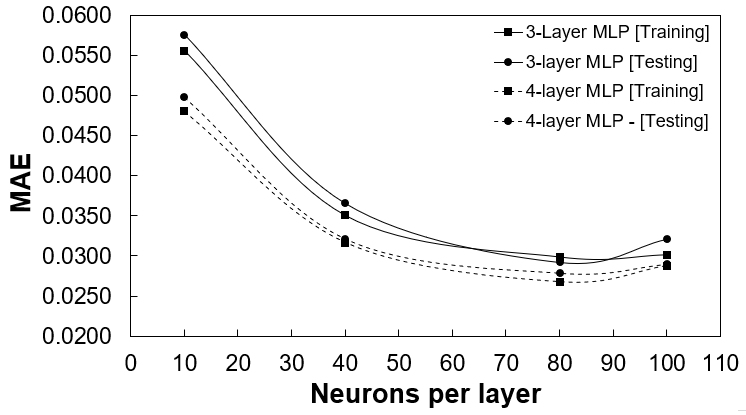
\includegraphics[width=1\textwidth]{NEURONS_HYPER}
    \caption{}
    \end{subfigure}\\
        \begin{subfigure}{0.5\textwidth}
    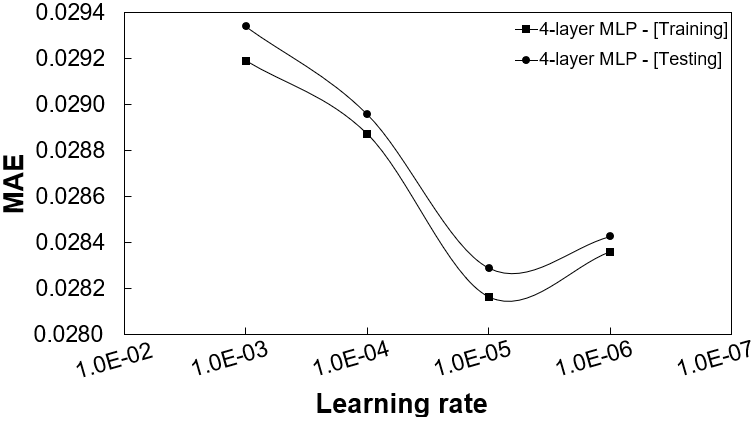
\includegraphics[width=1\textwidth]{LR_HYPER}
    \caption{}
    \end{subfigure}
        \begin{subfigure}{0.5\textwidth}
    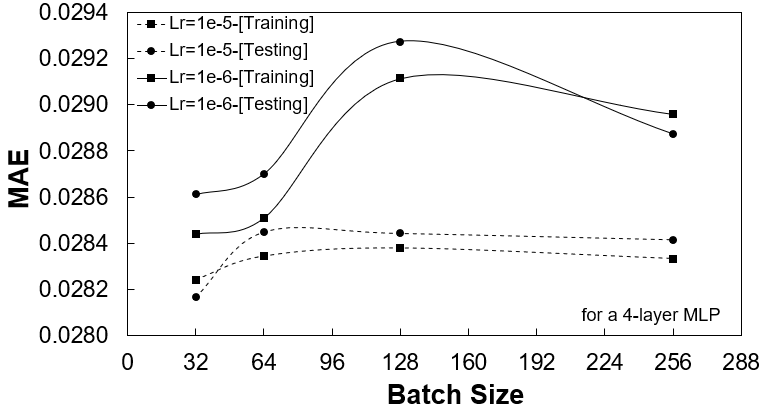
\includegraphics[width=1\textwidth]{BATCH_SIZE_HYPER}
    \caption{}
    \end{subfigure}
    \caption{MLP model performance for; (a) hidden layer architecture, (b) varying learning rates, and (c) varying mini-batch sizes}\label{fig_mlp_hyper}
\end{figure}

The MLP-MDN hyper-parameter tuning was conducted in a similar manner only that an additional step was required. This was to consider the number of distributions the MLP-MDN would use to capture the probabilistic characteristics. Figure \ref{fig_mdn_hyper} shows the MAE for the various distributions, with a distribution of 1 representing the best MLP model. An increase in the number of distributions tends to improve the MAE, however it is evident that a threshold of 3 distributions results in the best improvement.\\
\begin{figure}[h!]
	\centering
		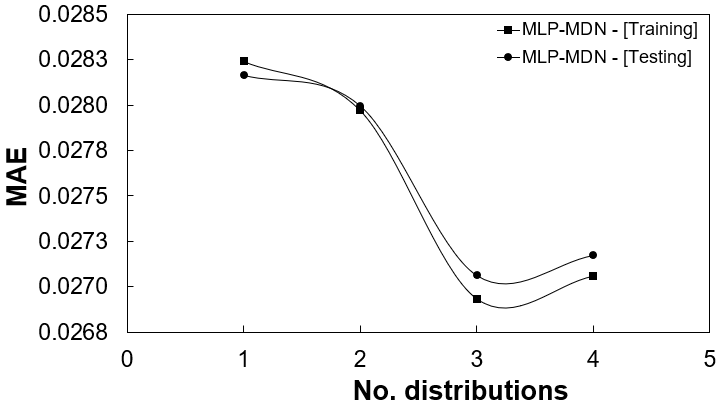
\includegraphics[width=0.5\textwidth]{DIST_HYPER}
	  \caption{MLP-MDN model performance for number of distributions}\label{fig_mdn_hyper}
\end{figure}

The results of hyper-parameter search are given in Table \ref{tbl_hyper_results}. Unlike the MLP, which can only produce a single set of predictions for an input, the MLP-MDN is able to produce a distribution of predictions based on the most probable mixing coefficient. This highlights one of the main advantages of the using the MLP-MDN model is its ability to learn the uncertainty that comes from using a probabilistic model. This is shown in the error distributions graphs of Figures \ref{fig_frequency_data} (a) and (b) with addition of uncertainty on the percentage error is introduced. A simple linear regression model was used as a base model for comparative purposes. For the MLP-MDN model it is seen that approximately 80-90\% of the training data has mean absolute percentage errors (MAPEs) below 10\%, with the MLP model showing a similar trend. Both models show considerable improvement in comparison to the linear model.\\

Based on the above analysis, the MLP-MDN model was selected as the best model to be used for the surrogate model implementation. As mentioned, the MLP-MDN model is able determine the uncertainty associated with each prediction, an important feature for future investigations incorporating transient/dynamic responses.

\begin{table}[h!]
\caption{Hyper-parameter search results}\label{tbl_hyper_results}
\begin{tabular*}{\textwidth}{lp{0.4\textwidth}l}
\toprule
 Parameter& MLP & MDN-ANN \\ % Table header row
\midrule
 Number of distributions & - & 3  \\
 Number of layers & 4 & 4\\
 Number of neurons per layer & 80  & 80\\
 Learning rate & 1e-5 &  1e-5   \\
 Mini batch size  &32 & 32  \\
\midrule
Errors & &\\
\midrule
RMSE & 0.0213 & 0.0211\\
MAE & 0.0282& 0.0263\\
\bottomrule
\end{tabular*}
\end{table}  

\begin{figure}[h!]
\centering
    \begin{subfigure}{0.5\textwidth}
    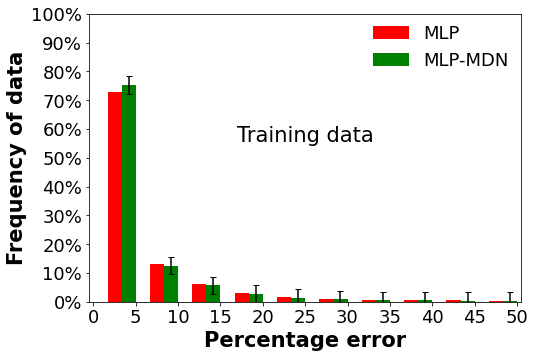
\includegraphics[width=1\textwidth, height =5.5cm]{OVERALL_TRAIN}
    \caption{}
    \end{subfigure}\\
    \begin{subfigure}{0.5\textwidth}
    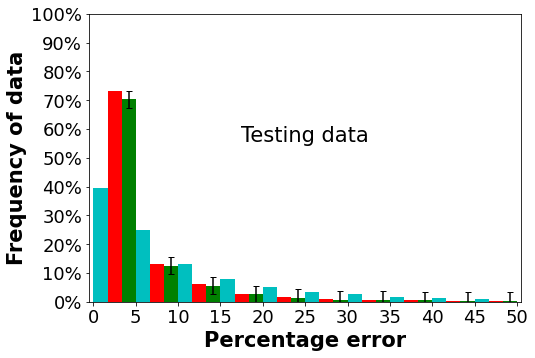
\includegraphics[width=1\textwidth, height =5.5cm]{OVERALL_TEST}
    \caption{}
    \end{subfigure}
    \caption{Error distributions for the selected MLP and MLP-MDN model h; (a) training data and (b) testing data}\label{fig_frequency_data}
\end{figure}

\subsection{Process model integration}
The validation and the subsequent case-studies of Section \ref{sec_results_diss}, make use of an integrated surrogate and network based 1D process model. The process model is used to capture the thermodynamic response of the water/steam side of the utility boiler under investigation, with the developed data-driven surrogate model (i.e. MLP-MDN) providing the gas-side thermal predictions and heat-exchanger heat loads.\\

A C\# script is used to access the Python application programming interface (API) available in the process modelling software, Flownex SE\textsuperscript{\textregistered} 2021. This allows for predictions to be made using the trained MLP-MDN model. The most probable predictions are retrieved using the script and transferred to the respective process model components as inputs. A schematic of the surrogate and process models integration is provided in Figure \ref{fig_int_model}.\\
\begin{figure*}[h!]
	\centering
		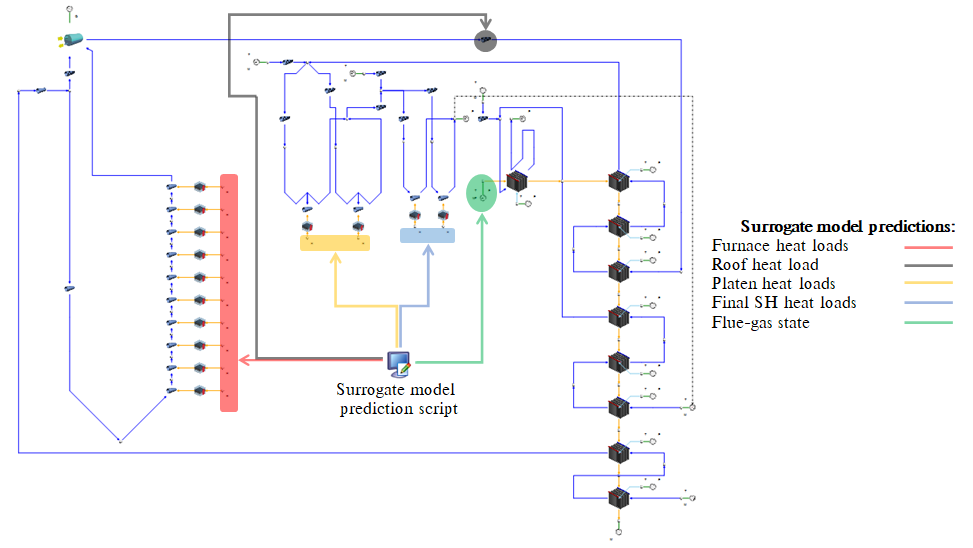
\includegraphics[scale=0.15]{INTEGRATED_MODEL}S
	  \caption{Schematic of integrated surrogate and network based process model}\label{fig_int_model}
\end{figure*}

The boiler can be split into three sections namely, the furnace, the radiative pass consisting of the platen (SH2) and final (SH3) SHs, and the convective pass consisting of the secondary re-heater (RH2), primary SH (SH1), primary re-heater (RH1) and the economizer (ECO). The furnace heat load predictions to the furnace walls determine the evaporation rate. The high pressure (HP) steam outlet steam flow rate is calculated as the addition of the attemperation flow rates (ATT1 and ATT2) and the evaporation flow rate. The attemperators are used to control the steam temperature to ensure an exit temperature of $808K$ at both the HP outlet and RH outlet. In addition to the furnace heat loads the surrogate model predicts the platen and final SH heat loads. Lastly the surrogate model is able to predict the flue-gas conditions at the inlet to convective pass (i.e. RH2). The furnace walls, platen and final SHs are represented by a single lumped parameter pipe flow component, interconnected with nodes that introduce the attemperation flows to the water/steam side. The convective pass components are modelled using an in house heat exchanger model that accounts for the radiative (gas and direct), convective and conduction heat transfer mechanisms to and from the gas-side and steam-side control volumes, as well as between the up- and downstream heat exchangers on the gas side.

\section{Results and discussion}\label{sec_results_diss}
As concluded in Section \ref{sec_hyper}, the MLP-MDN model is used for the surrogate model integration. The subsequent sections provide a validation of the integrated models thermal response and a case study that investigates the effects of using poor quality fuel. 

\subsection{Multiple load validation}\label{sec_result_1}
The surrogate models predictions and thermal-hydraulic response are validated for 100\%, 80\% and 60\% MCR load cases. The measured plant data for the respective load ratings were made available, allowing for the mean and standard deviation to be calculated from the plant data, thus capturing the uncertainty of the measurement devices used in the plant.\\ 

The benefit of using the MLP-MDN surrogate model is its ability to provide predictions along with  its respective standard deviation. To incorporate the prediction/s uncertainty and propagate this through the entire integrated model, the current work made use of the Monte Carlo method \cite{Thomopoulos2013}. The method is used to illustrate how a model responds to randomly generated inputs, the process is described as follows process. Firstly random sampling of the input variable/s (in this case the MLP-MDN model predictions) are performed based on the mean and standard deviation to produce $N$ number of scenarios, secondly simulations are run for each scenario, finally ongoing assessment of the simulations results are performed on measures such as the mean and standard deviation.\\ 

The use of Flownex SE\textsuperscript{\textregistered} 2021s built in Monte Carlo method, requires the mean and standard deviation for the inputs that are to be varied \cite{flownex}. For this study $N$=1000 scenarios where performed for each validation case with the mean and standard deviation being used as measures to determine convergence. The MLP-MDN input vectors ($\overline{X}$) for the validation cases are provided in Table \ref{tbl_inputs}, these inputs were obtained from the works of Laubscher and Rousseau \cite{Laubscher2019b}.\\

\begin{table*}[h!]
\caption{MLP-MDN input vectors ($\overline{X}$) for the validation and varied fuel case studies}\label{tbl_inputs}
\begin{tabular*}{\tblwidth}{lp{0.12\textwidth}p{0.12\textwidth}p{0.12\textwidth}p{0.12\textwidth}p{0.12\textwidth}}
\toprule
 & \multicolumn{3}{c}{\textbf{Validation load cases}}&\multicolumn{2}{c}{\textbf{Varied fuel load cases}}\\
\textit{Inputs}& 100\%  & 80\% & 60\% & High-ash & High-moisture  \\
\midrule
Excess air ratio - [-] & 1.155 & 1.209 & 1.263 & 1.155 & 1.155  \\
$Y_{ASH}$ - [$kg/kg$] & 0.409 & 0.409 &  0.409 &0.5 & 0.409  \\
$Y_{H_{2}O}$ - [$kg/kg$] & 0.055 & 0.055 & 0.055 & 0.055 & 0.146  \\
HHV = $f(Y_{ASH},Y_{H_{2}O})$ - [$MJ/kg$] & 15.07 & 15.07 & 15.07 & 12.68 & 12.68  \\
Platen SH fouling - [$K/W$]& 0.012 & 0.012 & 0.012 & 0.012 & 0.012  \\
Final SH fouling - [$K/W$] & 0.0067&0.0067 &0.0067 & 0.0067&0.0067  \\
Total fuel flowrate - [$kg/s$] &108.6 & 90.72 & 60.12 &108.6 & 108.6 \\
Platen SH mean steam temp. - [$K$] & 698 &697&781 &698 &698  \\
Final SH mean steam temp. - [$K$]& 787 & 793 &781 &787 &787  \\
\bottomrule
\end{tabular*}
\end{table*}  
\begin{figure*}
\centering
\begin{subfigure}{0.33\textwidth}
    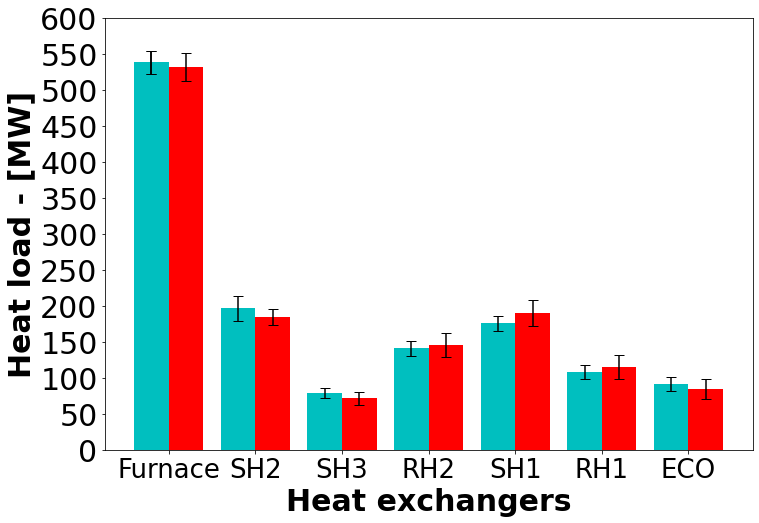
\includegraphics[width=\textwidth, height = 4.25cm]{100_CASE}
    \caption{100\% MCR}
\end{subfigure}\hfill % maximize horizontal separation
\begin{subfigure}{0.33\textwidth}
    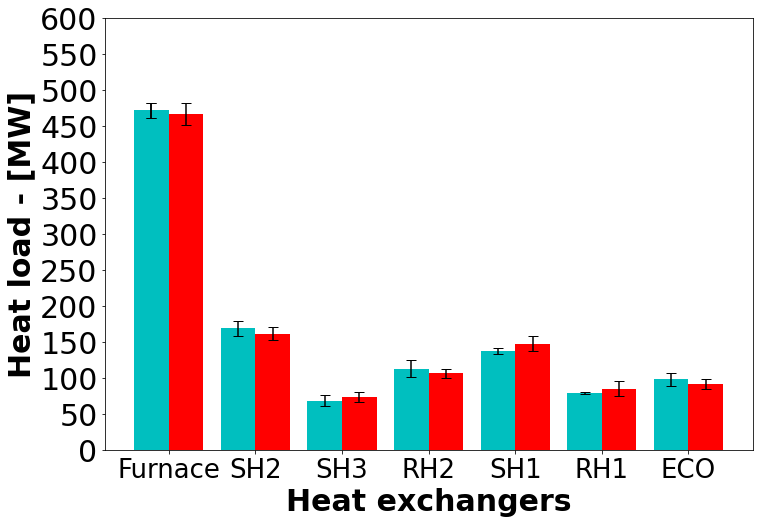
\includegraphics[width=\linewidth, height = 4.25cm]{80_CASE}
    \caption{80\% MCR}
\end{subfigure}\hfill
\begin{subfigure}{0.33\textwidth}
	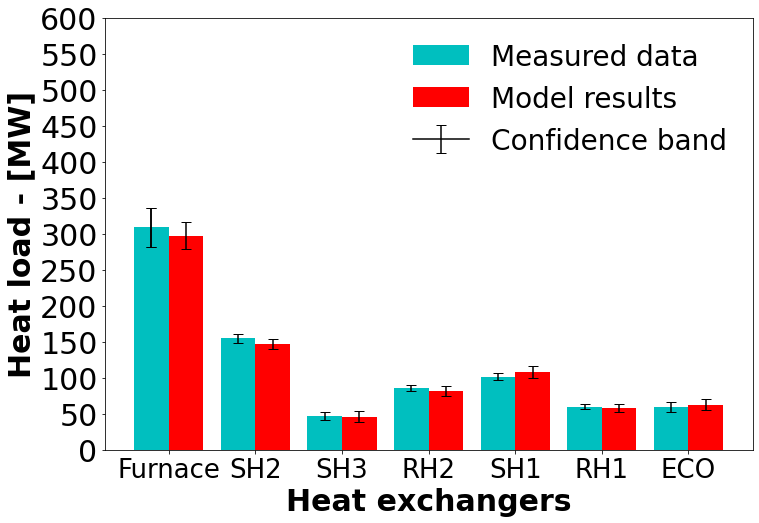
\includegraphics[width=\linewidth, height = 4.25cm]{60_CASE}
        \caption{60\% MCR}
\end{subfigure}
\caption{Load validation result comparison of the measured data and MLP-MDN model results for the various heat exchangers}
\label{fig_heat_load}
\end{figure*}

\begin{figure*}
\centering
\begin{subfigure}{0.33\textwidth}
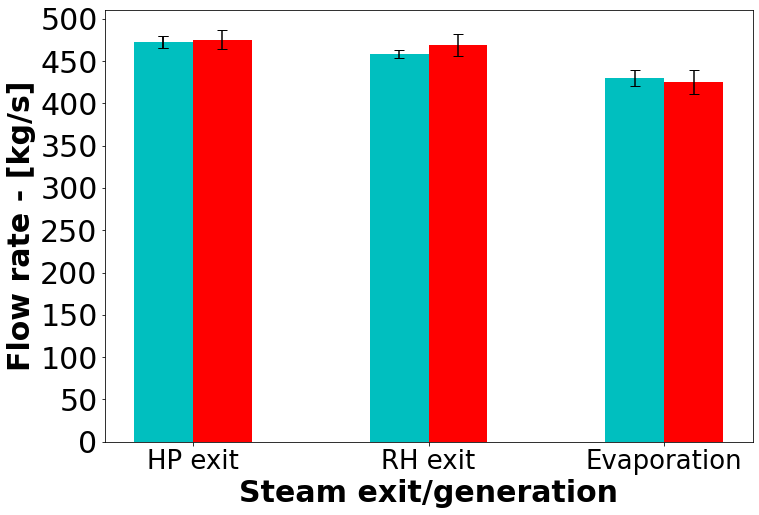
\includegraphics[width=\linewidth, height = 4.25cm]{100_CASE_STEAM}
        \caption{100\% MCR}
\end{subfigure}\hfill % maximize horizontal separation
\begin{subfigure}{0.33\textwidth}
    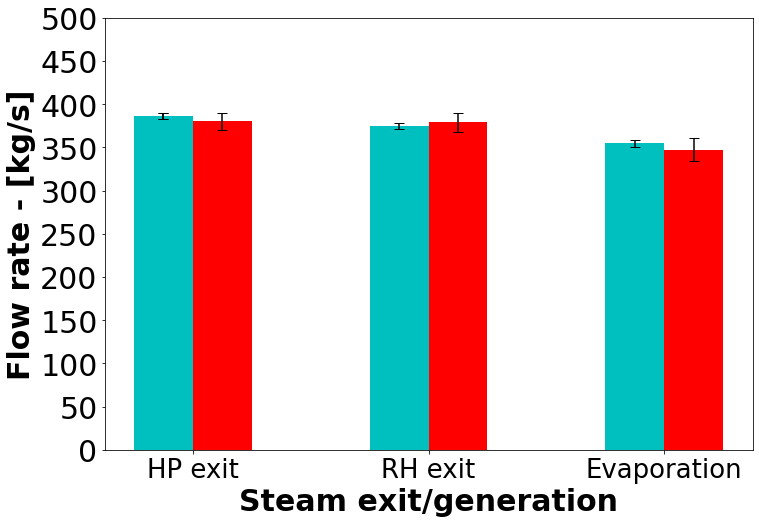
\includegraphics[width=\linewidth, height = 4.25cm]{80_CASE_STEAM}
    \caption{80\% MCR}
\end{subfigure}\hfill
\begin{subfigure}{0.33\textwidth}
	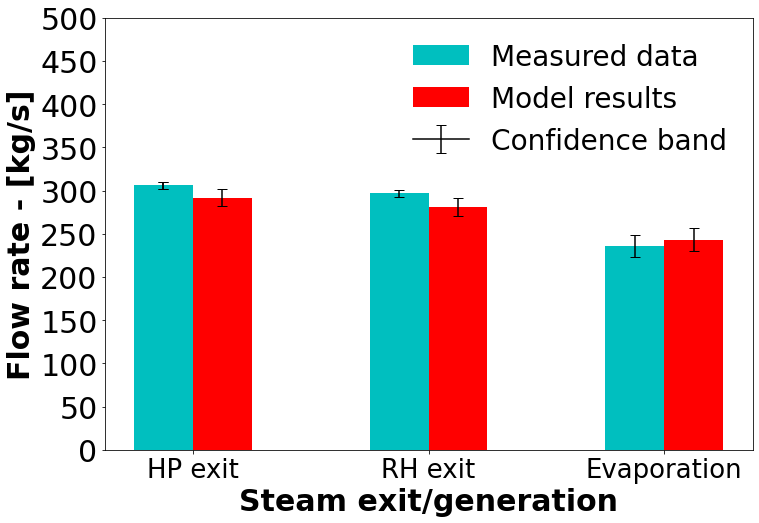
\includegraphics[width=\linewidth, height = 4.25cm]{60_CASE_STEAM}
    \caption{60\% MCR}
\end{subfigure}
\caption{Load validation result comparison of the measured data and MLP-MDN model results for the steam exit and generation flowrates}
\label{fig_steam_gen}
\end{figure*}

\begin{figure*}
\centering
\begin{subfigure}{0.33\textwidth}
    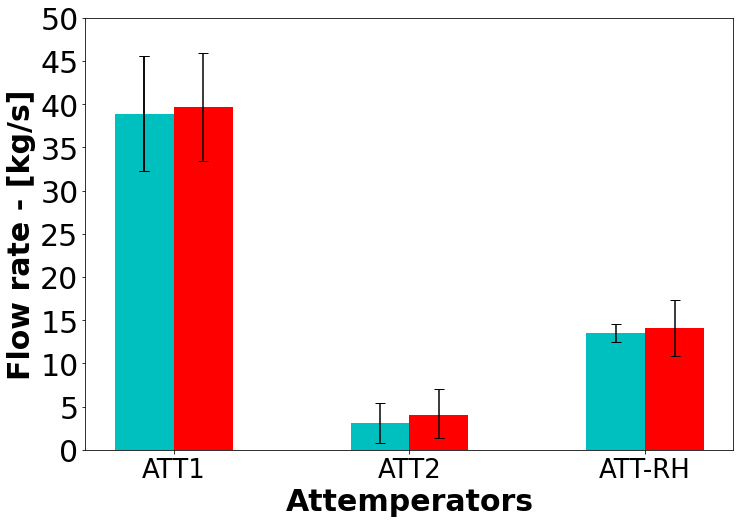
\includegraphics[width=\linewidth, height = 4.25cm]{100_CASE_ATTEMP}
    \caption{100\% MCR}
\end{subfigure}\hfill % maximize horizontal separation
\begin{subfigure}{0.33\textwidth}
    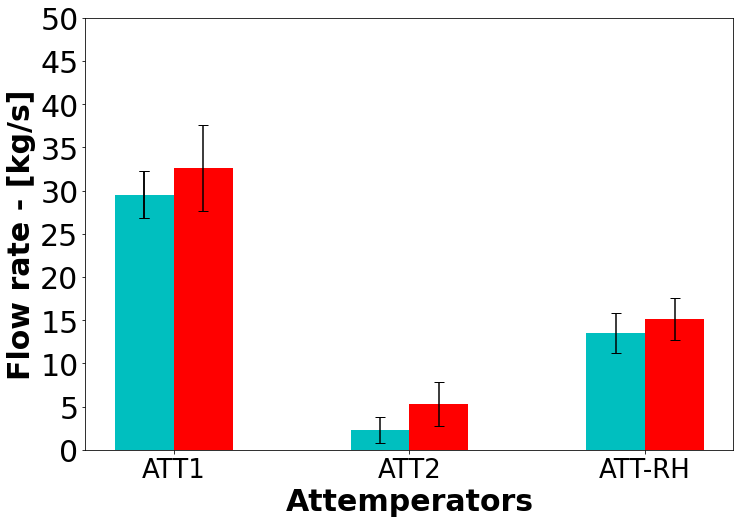
\includegraphics[width=\linewidth, height = 4.25cm]{80_CASE_ATTEMP}
    \caption{80\% MCR}
\end{subfigure}\hfill
\begin{subfigure}{0.33\textwidth}
    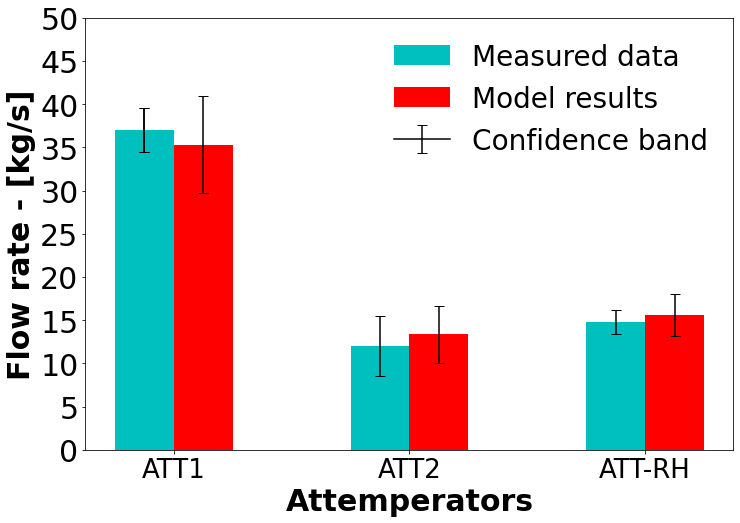
\includegraphics[width=\linewidth, height = 4.25cm]{60_CASE_ATTEMP}
    \caption{60\% MCR}
\end{subfigure}
\caption{Load validation result comparison of the measured data and MLP-MDN model results for the required attemperator flowrates to maintain operational integrity}
\label{fig_attemp}
\end{figure*}

Figures \ref{fig_heat_load} - \ref{fig_attemp} provide comparative results of the measured data and integrated model responses for all three load cases. It can be seen for a range of MCR loads the integrated model is able capture the heat loads to the various heat exchangers (Figures \ref{fig_heat_load} (a-c)) with sufficient accuracy. In general the model under-predicts the mean of the heat loads in the furnace and radiative pass, with slight over-predictions seen in the convective pass. However, the associated uncertainty of the integrated model overlaps with the measured data uncertainty with minimal outliers.\\ 

Considering the steam generation and exit flowrates of Figure \ref{fig_steam_gen} (a-c), it can be seen that the integrated model is able to sufficiently capture the hydraulic response of the case study boiler for a wide range of loads. A higher degree of uncertainty is associated with the integrated model but this is deemed acceptable since the response overlaps with the measured data. The attemperators of a utility scale boiler, are an integral part of the control systems put in place to ensure safe operating conditions and minimal wear on the downstream components, namely the steam HP and Low-pressure steam turbines \cite{Kakac1991}. Figure  \ref{fig_attemp} (a-c) highlight the attemperator flowrates across a wide range of loads. The integrated model is shown to adequately resolve the flowrates with a slightly higher mean being predicted for the 80\% load case.\\

It has been shown that integrated model is able to resolve the thermal response based on the predictions of the MLP-MDN model for a wide range of loads with sufficient accuracy. The heat loads are within a 5\% tolerance of the measured data's mean value, while the steam generation rates exhibit a maximum difference of 7\%, which seen in the 60\% MCR load case (refer to Figure \ref{fig_steam_gen} (c)). The attemperators results feature the largest uncertainty/confidence band of all the results (Figure \ref{fig_attemp}), however the confidence bands do overlap within 5\%. 
\subsection{Utility boiler response for a fuel with high ash \& moisture contents}
The following section makes use of the validated model of Section \ref{sec_result_1}. The fuel constituents that effect the energy content of the fuel (HHV) the most are primarily the ash ($Y_{ASH}$) and moisture ($Y_{H_{2}O}$) content. Thus, two case studies were made to illustrate the effects of using poor quality fuel.\\

The input vectors for the two fuel cases are provided in Table \ref{tbl_inputs}, it can be seen that the all the inputs are identical to the 100\% load case except for the ash, moisture and higher heating value of the respective fuels. This was done to compare the effects of the poor quality coal to that of the 100\% load case, in terms of the boiler efficiency, heat pick-up and thermal response. It is important to note that both the high ash and moisture case studies have the same HHV value, thus allowing for a productive correlation of the results.\\

As with validation case studies of Section \ref{sec_result_1}, the Monte Carlo method was employed to ascertain the integrated models uncertainty for all responses. The base model heading of Figure \ref{fig_fuel_results} (a-c) refers to the integrated model results for the 100\% load case of Figures \ref{fig_heat_load}-\ref{fig_attemp}. Figure \ref{fig_fuel_results}  (a) highlights the effects that poor quality fuel have on the heat load to the various heat exchangers, with a 20\% drop being observed. This is an expected result since the energy content of the fuel is lower than that of the base case. To maintain 100\% load capabilities using the poor quality fuel an increase in the fuel flowrate would be suggested, this provides more energy content, however the mill operational outputs are limited. The operational protocol for the 100\% load case makes use of 5 mills operating 30 of the 36 burners, at full capacity with a standby mill and burner arrangement placed in reserve to help mitigate operational risks, such as maintenance schedules. Using the the standby mill would allow the fuel flowrate to increase by maximum 17\% , yet this would decrease the operational integrity and increase the associated risks. Since when burning the high-ash content fuel the likelihood of ash deposition/fouling of the heat exchanging components increases.\\

Figure \ref{fig_fuel_results} (b-c) similarly illustrates a decrease in the water/steam flowrates for the steam exit and attemperator conditions. The generation rates exhibit similar characteristics to the the 80\% load case of Figure \ref{fig_steam_gen} (b), illustrating a significant decrease in the operational capabilities when using a poor quality fuel. The predicted flue-gas temperatures entering the the convective pass are shown in Table \ref{tbl_fuel_results}. It is shown that for an increase in the fuels ash content the inlet temperature increases, which results in a higher radiative heat transfer percentage for the convective pass components (table \ref{tbl_fuel_results}). While the presence of more moisture in the fuel results in a lower inlet temperature, primarily due to the fact that the extra moisture requires a higher heat rate of evaporation, leading to lower radiative heat transfer percentages. Where the radiative heat transfer percentage per component $i$ is defined as follows: \\
\begin{equation}
\dot{Q}_{rad,i}\% = \frac{\dot{Q}_{rad,i}}{\dot{Q}_{rad,i}+\dot{Q}_{conv,i}}\times 100
\end{equation}

The boiler efficiency is the measure used to convey how well the combustion heat is transferred to the working fluid, and is defined as the ratio of total amount of heat absorbed by the heat exchangers (i.e. sum of the furnace, radiative and convective pass heat loads) and the combustion energy released ($m_{fuel}HHV$). A significant decrease in the boiler efficiency is highlighted in Table \ref{tbl_fuel_results}, for both fuel cases with the high ash fuel showing a slightly better result. The higher efficiency of the high-ash fuel is attributed to the fact that in general the heat loads to various heat exchangers are higher than that of the high-moisture fuel, this can be seen in Figure \ref{fig_fuel_results} (a). 

\begin{table}[h!]
\caption{Model results for poor fuel characteristics}\label{tbl_fuel_results}
\begin{tabular*}{\textwidth}{p{0.3\textwidth}p{0.2\textwidth}p{0.2\textwidth}p{0.2\textwidth}}
\toprule
\textit{Variable}& Base & High-ash & High-moisture \\ % Table header row
\midrule
Mean boiler efficiency [\%]& 88.2 & 77.6 & 75.9\\
Convective pass inlet flue-gas temp. [$K$]& 1352 & 1368 & 1311\\
\midrule
\multicolumn{4}{l}{\textit{Radiative heat transfer percentage (Convective pass)} }\\
\midrule
RH2 & 52.3& 56.2 & 50.3\\
SH1 & 46.3& 49.8& 47.2\\
RH1 & 21.3& 26.7& 18.2\\
ECO & 6.7& 8.3& 5.4\\
\bottomrule
\end{tabular*}
\end{table}  

\begin{figure*}
\centering
\begin{subfigure}{0.33\textwidth}
    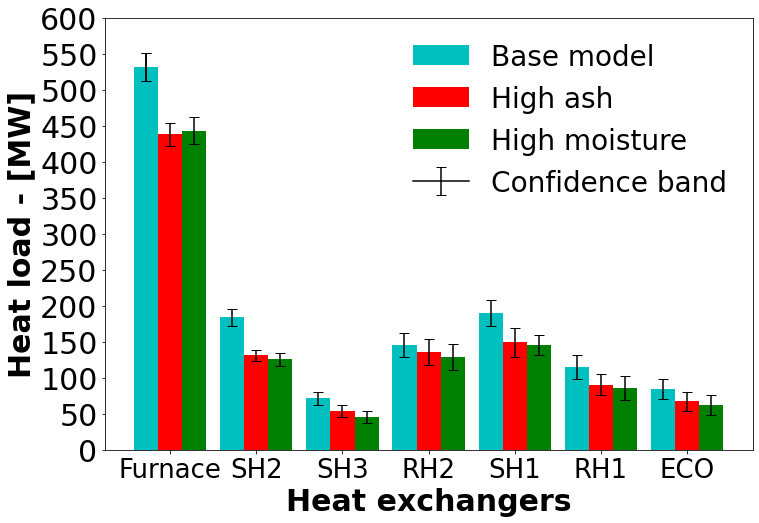
\includegraphics[width=\textwidth, height = 4.25cm]{100_FUEL_CASE}
    \caption{}
\end{subfigure}\hfill % maximize horizontal separation
\begin{subfigure}{0.33\textwidth}
    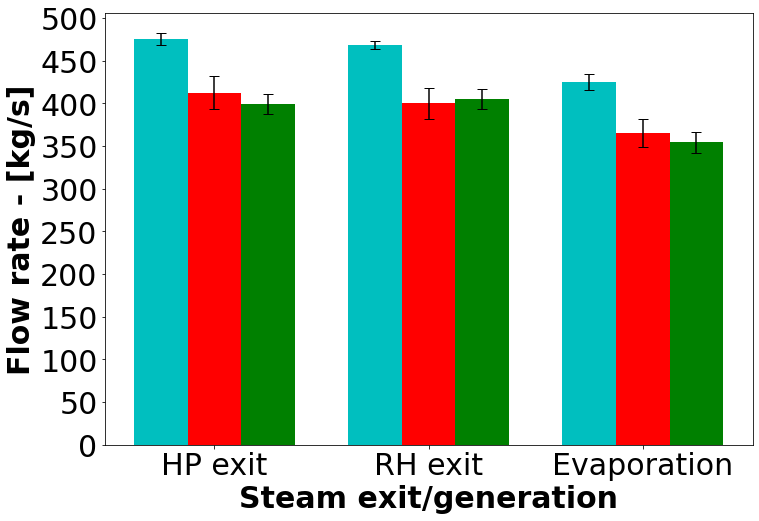
\includegraphics[width=\linewidth, height = 4.25cm]{100_FUEL_CASE_STEAM}
    \caption{}
\end{subfigure}\hfill
\begin{subfigure}{0.33\textwidth}
    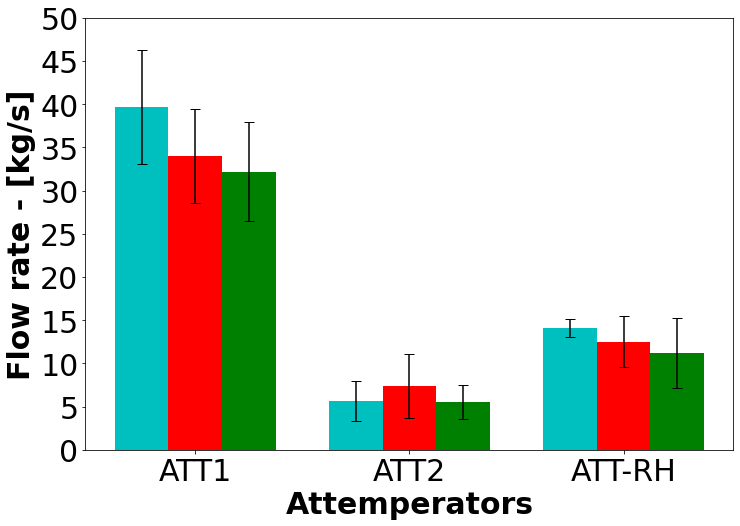
\includegraphics[width=\linewidth, height = 4.25cm]{100_FUEL_CASE_ATTEMP}
    \caption{}
\end{subfigure}
\caption{Integrated base, high-ash and high-moisture case study comparison for; (a) the various heat exchangers, (b) the steam exit and generation flowrates, and (c) the required attemperator flowrates to maintain operational integrity}
\label{fig_fuel_results}
\end{figure*}

\section{Conclusion}
The present work establishes the basis for utilizing an integrated data-driven surrogate and 1D process model to investigate the operational response for a 620 $MW_e$ utility scale boiler.\\

A data-driven surrogate modelling approach for a utility scale boiler using CFD simulations was presented that can predict the various parameters needed to capture the combustion heat transfer characteristics. These include the heat loads to the furnace and radiative pass components, and the flue-gas characteristics entering the convective pass, which include predictions of the temperature, species mass fractions and the radiation intensity. Training and testing datasets were generated using a 3-dimensional (3D) CFD model of the 620 $MW_e$ utility scale boiler under investigation. A total of 180 different CFD simulation cases were performed, where the input variables of Table \ref{tbl_doe} were varied.\\

It was found that the best surrogate model architecture was the use of a MLP-MDN configuration, allowing for uncertainty to be predicted. The configuration comprised of a MLP-MDN network consisting of 4 hidden layers each containing 80 neurons and 3 normal output distributions while using a learning rate of $1\times10^{-5}$ and batch size of 32. The MLP-MDN network illustrated that approximately 80-85\% of the model predictions had MAPEs below 10\%. The added benefit was the prediction of the uncertainty.\\

A validation case study was performed using the integrated model for a wide range of operational loads. The model results were compared to the measured thermal response for all load cases. The resolution of the heat loads, steam flowrates and attemperation flowrates resulted in a maximum error discrepancy of 7\%, highlighting the models sufficient accuracy of the key parameters. Using the Monet Carlo method the uncertainty predictions could be diffused through the integrated model, adding valuable insight into the operational limits of the model.\\

The subsequent analysis results investigated the using of poor quality fuels at 100\% MCR operation. The results highlight the drop in performance due to the fuel quality resulting in a substantial decrease in boiler efficiency. Using a high-ash fuel can result in a higher exit flue-gas temperature resulting in a marginal increase in performance of the convective pass heat exchangers when compared to the high moisture fuel. However the increase in particle loading increases the likelihood of ash deposition occurring.\\ 

The current work has shown that it is possible to adequately resolve the thermal-hydraulic response of a utility scale boiler using a data-driven surrogate model based off of CFD simulation result data. The integration of the surrogate and 1-D process model is paramount in modelling the thermal response and provides valuable operational insight for various load cases. The use of the model also provides a fast turn around and significant reduction in computational time when compared to co-simulation models using a combination of CFD and process modelling.
\printcredits
%% Loading bibliography style file
\bibliographystyle{model1-num-names}
%\bibliographystyle{cas-model2-names}

% Loading bibliography database
\bibliography{ML_paper}


\end{document}


